% Drawing 74/07-10 -- folder 74, batch 07, archive page 133 (PDF page 134).
% Transcription: un hexagone dont la moitié inférieure est en trait épais, avec un « W » inscrit ; trois rangées de points.
% Kind: hexagon with inscribed W; rows of points. Method 2 (schematic redraw from the facsimile). Status: ok.
% Notes: Hexagon whose lower half is in thick strokes, a W inscribed; at the right, rows of points (one big).
% Coordinates: 1 unit = 1 mm = 1/100 of the crop width (bbox in page fractions: [0.66, 0.475, 0.87, 0.545]).
% Redrawn by Claude (claude-opus-5-5), issue #73, 2026-11-07; not checked by a human; not compiled (no TeX in the session).
% Rights: reproduces part of the work -- behind RENDER_TRANSCRIPTS, never published by itself.
\documentclass[tikz,border=3pt]{standalone}
\usepackage{amsmath,amssymb}
\usetikzlibrary{patterns,arrows.meta}
\tikzset{pencil/.style={black!45}, struck/.style={black!35}, mark/.style={circle,draw,inner sep=1.3pt}, pt/.style={circle,fill,inner sep=0.9pt}, opt/.style={circle,draw,fill=white,inner sep=1.1pt}}
\begin{document}
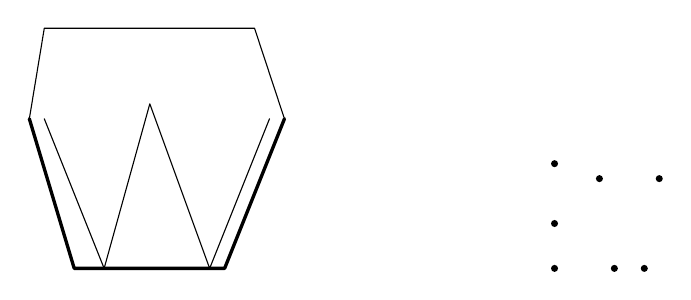
\begin{tikzpicture}[x=1mm,y=1mm,line cap=round,line join=round,font=\scriptsize]
\draw (9.5,-20) -- (11.4,-8.5) -- (38.1,-8.5) -- (41.9,-20);
\draw[very thick] (9.5,-20) -- (15.2,-39) -- (34.3,-39) -- (41.9,-20);
\draw (11.4,-20) -- (19,-39) -- (24.8,-18.1) -- (32.4,-39) -- (40,-20);
\node[pt,very thick] at (76.2,-25.7) {};
\node[pt] at (81.9,-27.6) {};
\node[pt] at (89.5,-27.6) {};
\node[pt] at (76.2,-33.3) {};
\node[pt] at (76.2,-39) {};
\node[pt] at (83.8,-39) {};
\node[pt] at (87.6,-39) {};
\end{tikzpicture}
\end{document}
